% Kelompok 4 Tugas GIS (WMTS)
% Hanna Tasya (!154091)
% Dhea Amelia (1154123)
% Yusri Rizal (1154072)
% Aji Muhammad Farhan (1154046)
% Tias Maulana (1154122)

\section{Web Map Tile Service}
Web Map Tile Service merupakan peta ubin yang dikembangkan pertama kali oleh Open Geospatial Constortium (OGC). 
Terdapat potensi di dalam Web Map Tile Services yaitu gambar peta ubin dapat di cache pada lokasi antara klien dan server, 
mengurangi latensi yang terkait dengan proses pembuatan gambar. Lapisan ubin biasanya di pasang di sisi server, menyajikan 
ubin gambar peta secara bersamaan ke beberapa pengguna. Selain itu, banyak pemetaan klien, seperti Google Earth atau Nasa 
World Wind, telah menyematkan cache, yang juga dapat mengurangi kemacetan jaringan dan penundaan jaringan. \cite{Garc{\'\i}a2002Web}

WMTS telah menjadi populer untuk visualisasi data geografis multi-dimensi di Internet. Dalam sistem tile, data disusun pada sejumlah 
skala yang telah ditentukan. Untuk setiap skala, area yang dipetakan dibagi menjadi banyak ubin persegi dengan ukuran 256 x 256 piksel.
Setiap ubin disimpan sebagai gambar di server Internet. Menggunakan ubin untuk memungkinkan visualisasi yang cepat di peta interaktif 
pada banyak skala ditunjukkan oleh Badan Penelusuran Angkasa dan Angkutan Udara Nasional (NASA) Global Cycle (Browse) 2013 di
http://earthdata.nasa.gov /labs / worldview / yang memberikan akses yang sangat responsif dan terukur terhadap citra real-time (Cechini
et al., 2013). Adopsi standar WMTS yang luas untuk penerbitan data salju diilustrasikan oleh katalog penelusuran ArcGIS Online 
(http://arcgis.com), di mana lebih dari 50 kumpulan data WMTS yang terkait salju dapat ditemukan. WMTS dapat diakses menggunakan browser 
web dan sistem informasi geografis (SIG). \cite{Kadlec2016Extracting} 


\subsection{Skema Ubin}
Peta sudah lama dikenal hanya seperti yang tercetak di atas kertas. Peta kartografi tercetak tersebut merupakan representasi 
statis yang terbatas pada skala visualisasi tetap dengan Tingkat Detil tertentu (LOD). Namun, dengan perkembangan peta digital, 
pengguna dapat memperbesar atau mengurangi area yang divisualisasikan dengan melakukan pembesaran operasi, dan LOD diharapkan 
dapat diperbarui sesuai dengan itu. 

Adaptasi konten peta sangat bergantung pada skala: Peta skala kecil berisi informasi yang kurang rinci daripada peta skala besar 
di wilayah yang sama. Proses mengurangi jumlah data dan menyesuaikan informasi dengan skala yang diberikan disebut generalisasi 
kartografi, dan biasanya dilakukan oleh server peta web.

Untuk menawarkan layanan peta web ubin, server peta web membuat peta melintasi serangkaian skala tetap melalui generalisasi yang 
progresif. Gambar peta yang dirender kemudian dibagi menjadi ubin, menggambarkan piramida ubin seperti yang digambarkan pada
gambar \ref{TilePyramid.JPG} 

\begin{figure}[ht]

\centerline{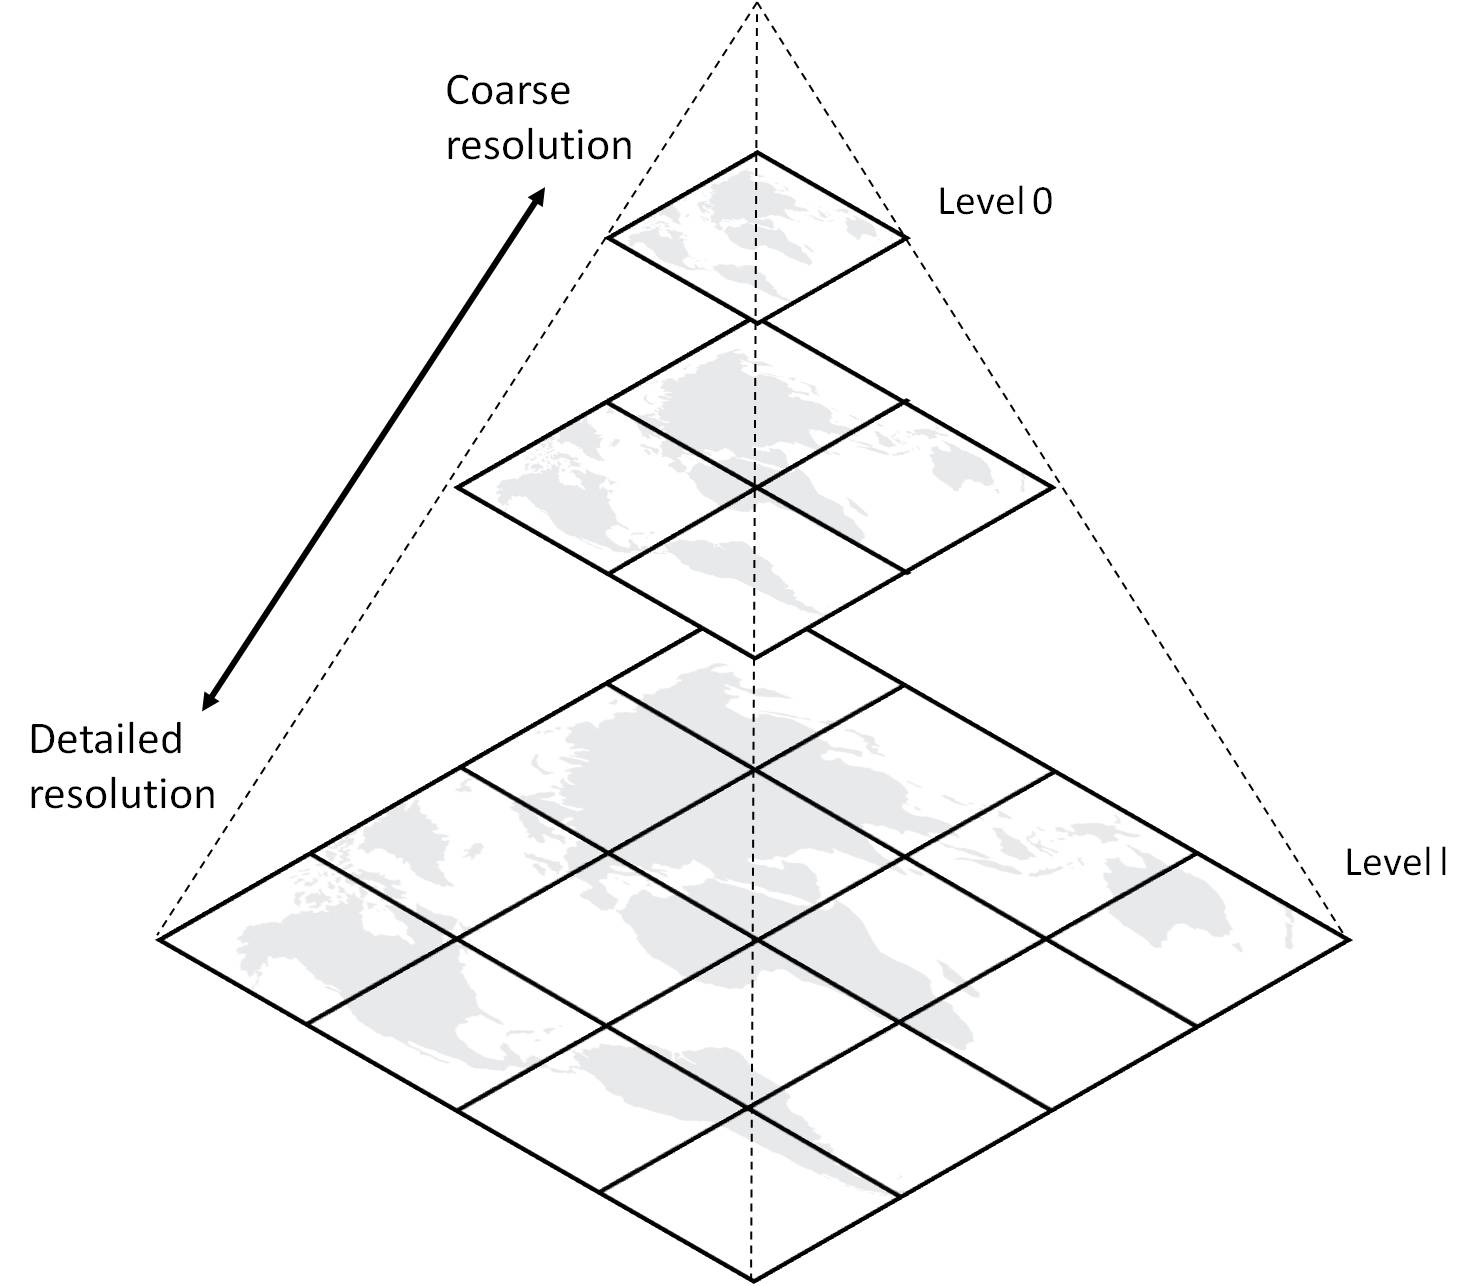
\includegraphics[width=1\textwidth]{figures/TilePyramid.JPG}}

\caption{Representasi piramida ubin}

\label{TilePyramid}

\end{figure}

gambar \ref{TilePyramid.JPG} merupakan contoh skema ubin dari Microsoft Bing Maps dimana tingkat pertama memungkinkan mewakili 
seluruh dunia dalam 4 ubin (2x2) dari  256x256 piksel. Tingkat berikutnya mewakili seluruh dunia dalam 16 ubin (4x4) dari 256x256 
piksel dan seterusnya sampai tingkat 4. \cite{Garc{\'\i}a2002Webmap}

\subsection{Metode Pemotongan Web Map Tiles Service}
Web GIS standar dibangun menggunakan WMS (Web Map Services). Ciri khas Web Gis dalam menampilkan data spasial atau mapadalah menarik 
langsung dari server dengan tidak memperhitungkan banyaknya lapisan yang diminta. Padahal proses menampilkan data spasial atau map ini 
tidak bisa dipaksakan menarik dalam jumlah besar karena akan memperlambat waktu respon web. Hal ini berbanding terbalik dengan harapan 
pengguna akan Web GIS yang mudahdioperasikan, memiliki tampilan yang ramah, pengaksesan yang halus dan data cukup update atau mendekati 
near real time[7] (Yang, 2011). 

Pendekatan umum untuk meningkatkan waktu respon saat permintaan data spasial adalah dengan memotong map 
menjadi beberapa bagian kecil atau tiles.Metode pemotongan ini secara standar bisa dibuat dengan WMTS (Web Map Tile Service) atau di 
kenal dengan tiles tradisional.Pemotongan standar cukup bisa mengurangi beban server namun waktu respon web masih lambat. Hal itu 
menjadi masalah yang saat ini dihadapi oleh Web Gis E-Government Sistem Pemantauan Bumi Nasional (SPBN). Pengguna harus menunggu lama 
waktu respon web.Padahal banyak informasi penting yang disampaikan khususnya terkait tanggap bencana titik panas kebakaran hutan yang 
terjadi saat ini. Dengan melihat fakta-fakta di atas, Penelitian ini ingin menganalisis penggunaan tiling pada open source web GIS, 
metode inimempertimbangkan tile static dan dynamic map. Untuk menganalisa digunakan metode matematika, data hasil testing, statistik 
hasil pengujian dan membandingkan beberapa metode yang telah berkembang untuk meningkatkan performa web gis. Penulis berharap analisis 
ini dapat meminimalkan waktu respon dan meningkatkan pelayanan E-Government Sistem Pemantauan Bumi Nasional (SPBN). Oleh karena itu 
penulis melakukan studi \“Analisis Optimalisasi Web Gis Dengan Metode Tiling\”. Penelitian ini diharapkan dapat membantu memecahkan 
masalah diatas. \cite{dewioptimalisasi}

\subsection{Peta Jalan}
proses pemetaan bumi secara akurat sampai saat ini, melestarikan yang sangat terampil, wellequipped,dan individu terorganisir
perkelompok. Bertahun-tahun biasanya peran surveyor, kartografer, dan ahli geografi untuk memetakan dunia dengan tulisan di atas kertas
atau, sejak tahun 1960an, masuk komputer. Ekspedisi Lewis dan Clark ke peta Amerika Utara Barat, dan Lambton dan Ekspedisi Everest's
Great Arc untuk India,hanya dua episode terkenal dalam sejarah peta dan pembuatan peta. Setiap negara memiliki lembaga pemetaan nasional
yang didirikan bermuatan dengan menjaga agar peta nasional tetap akurat saat ini (misalnya, Survei Geologi AS dan Survei Ordnance
Inggris).

Pada tanggal 1 Mei 2000. Presiden AS Bill Clinton,mengumumkan penghapusan ketersediaan selektif dari sinyal GPS1 dan dengan demikian,
disediakan akurasi yang jauh lebih baik untuk biaya sederhana dan murah.yaitu penerima GPS Secara praktis, ini berhasil mungkin untuk
mendapatkan posisi penerima dengan akurasi 6 sampai 10 meter dalam kondisi normal,berbeda dengan kira-kira 100 meter sebelumnya. Upaya
untuk mengembangkan lokasi berbasis layanan mendahului pemberitahuan dan berdasarkan informasi dari mobile tiang telepon atau beacon
lainnya. Namun, metode ini tidak mendapatkan banyak pangsa pasar karena untuk kompleksitas teknis dan ketidakmampuan mereka untuk
memberikan cakupan universal. Sebaliknya, GPS memungkinkan pengembangan receiver murah dengan akurasi posisi yang baik, dan, pada
pertengahan-2001, adalah mungkin untuk membeli unit penerimasekitar US $ 100,3 penerima ini membantu lebih banyak orang daripada
sebelumnya mengumpulkan informasi tentang lokasi yang berbeda dan upload ke komputer mereka.

Namun sampai tahun 2002, ketika standar pertukaran (format eXchange GPS atau GPX) diterbitkan, dimanipulasi dan berbagi Informasi ini
merupakan tugas yang rumit diperlukan komputasi dan manipulasi data pengetahuan. Untungnya, kebanyakan penerima GPS pengembang dengan
cepat mengadopsi standar GPX,dan, pada tahun 2004, sudah menjadi hal biasa ketersediaan lokasi berkualitas tinggi informasi telah
memungkinkan pemetaan mass market berdasarkan penerima GPS terjangkau, komputer rumah,dan internet.\cite{haklay2008openstreetmap}. 


\subsection{Desain Ekstraksi Data WMTS}
Mengekstraksi data deret waktu dari WMTS terdiri dari empat langkah utama:
(1) membangun alamat pengenal sumber daya seragam (URL) dari gambar ubin yang tumpang tindih pada titik waktu tertentu, 
(2) mendownload gambar ubin, 
(3) temukan koordinat piksel yang sesuai dengan titik kepentingan di dalam gambar yang didownload,
(4) ubah warna piksel atau indeks warna piksel ke unit variabel yang teramati.

Keempat langkah ini diulang untuk setiap langkah waktu dalam deret waktu (Gambar 1).

Spesifikasi WMTS, yang juga dikenal dengan nama \"TMS\" (layanan peta ubin), adalah protokol layanan web untuk mengambil gambar peta ubin yang telah
didefinisikan oleh OGC (Maso et al., 2010). Permintaan WMTS ada dalam format:

½server=½layer=½time=½x=½y=½zoom:png


